\section{Experiment Design}
\label{sec:experiment}
In this section, we detail the experiment design and rationale for these decisions.

\subsection{Experiment Protocol}
We recruited participants from a United States college town using online ads, digital bulletins, social media posts, online newsletters and physical flyers in public spaces beyond campus. To ensure participant diversity, we prioritized non-students by selectively accepting them as we monitoring demographics.The study was framed as focusing on societal attitudes to avoid response bias. The college Institutional Review Board reviewed and approved this study.
% If a respondent self-identified as a student, we thanked them and informed them of our current priority for non-students, though some self-identified students were still accepted.

\begin{figure}[ht]
    \centering
    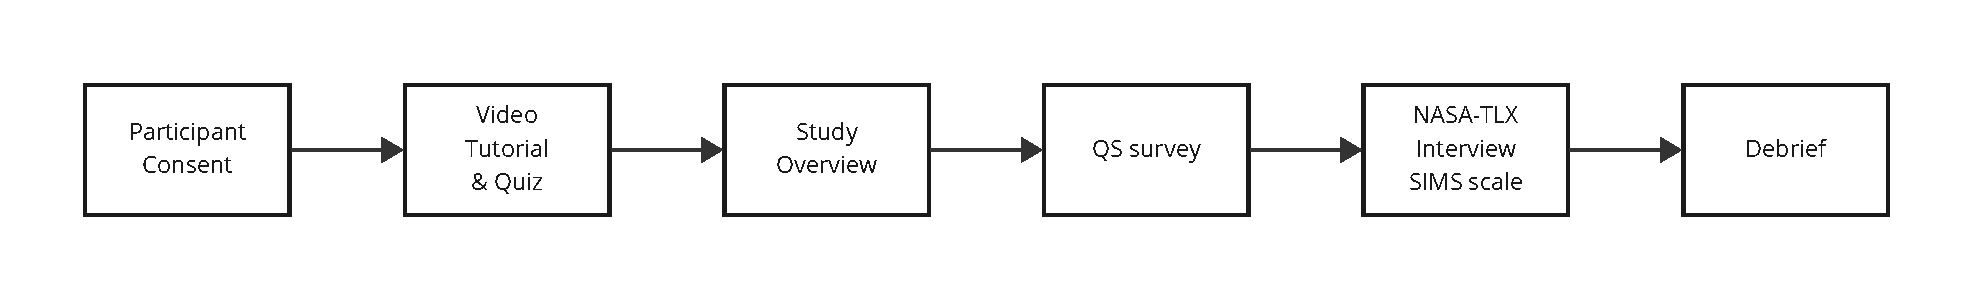
\includegraphics[width=1\textwidth]{content/image/study_flow.pdf}
    \caption{Study protocol: Participants are asked to learn about the mechanism of QS after consenting to the study. The researcher explains the study overview and asked participants to complete the QS. A NASA-TLX survey followed by interviews to understand participant's cognitive load. A debrief happens before ending the study.}
    \label{fig:studyProtocol}
\end{figure}

Figure~\ref{fig:studyProtocol} visually represents the study protocol. Participants completed the study in the lab to control for external influences. Participants used a 32-inch vertical monitor displaying all options on the survey to prevent hidden information during decision-making. After consenting, participants watched a video explaining the Quadratic mechanism without hints of interface operation followed by a quiz to ensure understanding. Participants rewatch the video or consult the researcher until they could select the correct answers. The participant's screen was captured throughout the study. The researcher primed the participant that the study aimed to help local community organizers understand preferences on societal issues to better allocate resources. Participants were randomly assigned to one of four groups:

\begin{itemize}
    \item 6 options with a text-based interface (ST)
    \item 6 options with an two-phase interface (SI)
    \item 24 options with a text-based interface (LT)
    \item 24 options with an two-phase interface (LI)
\end{itemize}

Participants completed the survey independently, without the researcher's presence. They then contacted the researcher for the NASA-TLX survey followed by a short audio recorded semi-structured interview. The session concluded with a debriefing and a \$15 cash compensation, during which participants were informed of the study goal on cognitive load and interface design.

\subsection{Experiment Design Choices}
This subsection explains the four experiment design decisions:

\subsubsection{A between subject study}
We chose a between-subject design to minimize study fatigue and avoid the learning effect. The complexity of QS survey made completing back-to-back studies impractical. Since preferences are constructed, we wanted to ensure that participants were not influenced by their previous preferences, which could affect their perceived cognitive load and decision-making process.

% asking participants to revisit the lab after several days would likely increase dropout rates and demotivate participants from attending in-person sessions. Second, we aimed to reduce the learning effect, which is challenging to eliminate, especially concerning interface operation and decision-making in the survey. 

\subsubsection{Deciding number of survey options}
Identify the `breaking point' for cognitive overload ideally requires testing a range of option numbers, but this was impractical due to time and resource constraints. Therefore, we relied on prior literature to test 6 and 24 options, representing short and long lists. Constant sum surveys and the Analytic Hierarchy Process (AHP) recommend fewer than ten and seven options, respectively~\cite{moroneyQuestionnaireDesignHow2019, saatyGroupDecisionMaking2013, saatyPrinciplesAnalyticHierarchy1987}.~\textcite{millerMagicalNumberSeven1956} classic work on cognitive processing capacity and~\textcite{saaty2003magic}'s theoretical proof supported the use of $7\pm2$ items. A meta-analysis by~\textcite{chernevChoiceOverloadConceptual2015}  identified 6 and 24 are common values for short and long lists in choice overload studies, rooted in the original experiment by~\textcite{iyengarWhenChoiceDemotivating2000}.% Thus, we adopted these values to align with prior research. \footnote{We believe that the original value decision was due to the limitations of the jam flavors.}

\subsubsection{Context of the Study}
Participants completed a societal issue survey, following the methodology from~\textcite{chengCanShowWhat2021}. Societal issues are relevant to all citizen and effectively illustrate the need to prioritize limited public resources. We curated $26$ societal issues used by Charity Navigator~\cite{CharityNavigator2023} which evaluates over $20,000$ charities in the United States. The interface randomly present options from this list to participants. Appendix~\ref{sec:charityList} contains the full list.

\subsubsection{Using NASA-TLX to measure cognitive load}
Cognitive load can be measured through performance measures, psychophysiological measures, subjective measures, and analytical measures~\cite{gaoMentalWorkloadMeasurement2013}. Given the extended nature of QS, performance measures using a secondary task were impractical. Psychophysiological measures such as pupil size~\cite{palinkoEstimatingCognitiveLoad2010} and ECG~\cite{haapalainenPsychophysiologicalMeasuresAssessing2010} were costly and sensitive to external factors. 

Therefore, we deployed self-report subjective surveys and analytical measures (i.e., like time and clickstream data). We adopted the paper-based weighted NASA Task Load Index (NASA TLX), a widely used multidimensional tool that averages six subscale scores to represent overall workload after completing a task~\cite{hart1988development, hartNasaTaskLoadIndex2006, cain2007review} Despite some criticisms, NASA-TLX is favored for its low cost, ease of administration~\cite{gaoMentalWorkloadMeasurement2013}, and significantly less variability compared to one-dimensional workload scores~\cite{rubioEvaluationSubjectiveMental2004}, making it suitable for our study.


% Finally, participants complete the situational motivation scale (SIMS) to gauge motivation and a demographic survey.
% Last, we describe the two quantitative measurements taken during the study: cognitive load and motivation. 
% , indicating differences in workload definitions among raters within a task and variations in workload sources between tasks

% Tabling SIMS for now. It was not used in the analysis. In addition to NASA-TLX, we administered a situational motivation scale (SIMS) to measure participants' motivation (required citation). We posited that motivation would influence mental demand (required citation). SIMS, chosen for its widespread use, helps understand one's intrinsic motivation, extrinsic motivation, identified regulation, and external regulation, and was originally designed to measure self-determination. Both instruments were administered using pen-and-paper.

% The reason we made this experiment design decision was to minimize . External factors, more prevalent in remote experiments or those conducted via platforms like MTurk, included potential multitasking or interruptions by others. An in-lab study also allowed participants to operate across a consistent device that researchers had full control over.